\afterpage{\blankpage}
\chapter{Experiments}
Given that at the core of the application are learning algorithms, the system reliability is determined by the databases from which train and test data is used. Although for the face embedding part we are not able to train the neural network ourselves given the limited computational power at our disposal, for the face validation part, the public domain databases offers us a large choice, the most commonly used ones are described in the following sections with the corresponding experiments. In order to learn the face distance threshold, we use another database, MS-Celeb-1M \cite{guo2016msceleb}, but given it's purpose for training neural networks, we only use a small sample which is enough to give us sufficient information about the optimum value of the parameter.


\section{Evaluation protocol}
In order to determine the quality of our implementation and to be able to compare it to other works, we use clear evaluation protocols for each database. For all of the experiments, in terms of determining the appropriate parameters for the SVM, we make a grid search over multiple values for each parameter. This grid search does a 3-fold cross validation over the training data and selects the parameters with the best results.
We report the results in terms of receiver operating characteristic curve (ROC curve), area under de curve (AUC), equal error rate (EER) and confusion matrix.

We create the \textbf{ROC curve} by plotting the true positive rate on the Y axis and false positive rate on the X axis. The ideal point is the top left which means a true positive rate of 1 and a false positive rate of 0. In practice this is not very realistic, but it does mean that a larger \textbf{area under the curve} is usually better. An important thing to notice is the "steepness" of the curve as it is desired to maximize the true positive rate while keeping at a low the false positive one.

A statistic we use to show biometric performance, typically when operating in the verification task is the \textbf{equal error rate (EER)}. It represents the error rate of a verification system when the operating threshold for the accept/reject decision is adjusted such that the probability of false acceptance and of false rejection become equal. 

Another method we use to describe the performance of our classification model is the confusion matrix. It represents a table that shows quantitative results of the predictions in relation to the ground truth. More precisely, it counts for every class the number of examples that were correctly classified and the number that were not. A two class example can be seen in Figure \ref{fig:confusion_matrix}.

\begin{figure}[H]
	\captionsetup{width=15cm,font=small}
	\begin{center}
		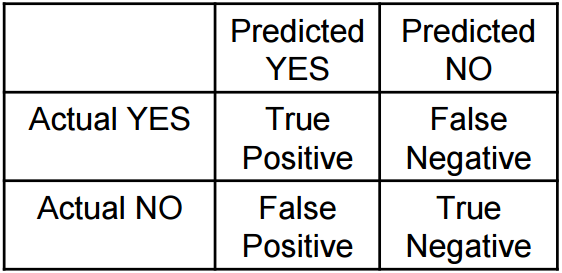
\includegraphics[width=10cm]{confusion_matrix}
	\end{center}
	\caption[Confusion matrix representation]{Confusion matrix representation. Lines correspond to ground truth given by known labels. Columns correspond to the predicted labels. Inside the matrix the corresponding number of examples are noted.}
	\label{fig:confusion_matrix}
\end{figure}

\section{Face spoof databases}\label{section:face_spoof_databases}
In this section we analyze the accuracy of our LBP-implementation of a face liveness linear SVM classifier method based on the most commonly used anti-spoof face databases available in public domain. We present our intra-database experiments as well as cross-database ones, the latter being considered better in modeling a real use case.
\subsection{CASIA face antispoofing database }
CASIA database for face antispoofing was created by the Center of Biometrics and Security Research (CBRS) and is composed by 600 videos divided in three categories: low, normal and high quality of 50 asian subjects, 12 videos for each. Out of the 12 videos, 3 are genuine and 9 are fake.
\begin{figure}[H]
	\captionsetup{width=15cm,font=small}
	\begin{center}
		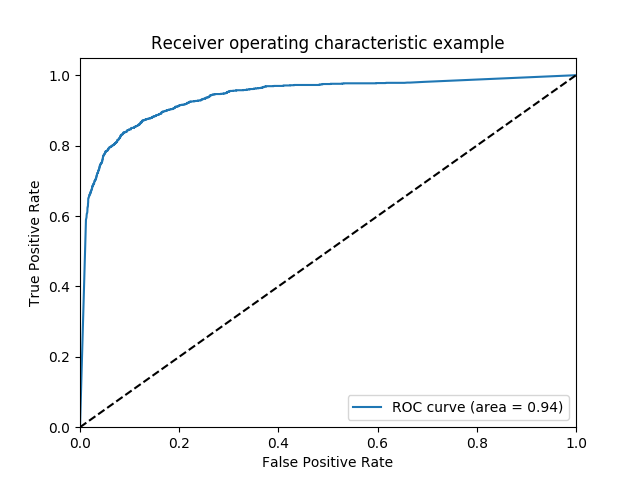
\includegraphics[width=10cm]{casia}
	\end{center}
	\caption[CASIA database reported ROC curve]{The resulted receiver operating characteristic curve for the Casia database corresponding to our implementation of a face spoof validator based on uniform LBP and linear SVM}
	\label{fig:casia_roc}
\end{figure}

There are implemented three face attacks which include: warped photo attack in which the printed photo is bended over the subjects face, cut photo where the eyes on the printed photo are cropped and then position on in front of the subject's face so that the blinking is made possible and video attack replayed on an IPAD.

We apply various evaluation methods for our face spoof classifier and for the CASIA database we report $0.938$ area under the receiver operating characteristic curve(ROC AUC), an equal error rate (EER) of $0.128$ and an accuracy score of $0.879$ based on the following confusion matrix
$
[
\begin{smallmatrix}
&Spoof & Real\\
Spoof & 4058 & 514\\
Real & 214 & 1262
\end{smallmatrix}], 
$. The ROC curve can be seen in figure \ref{fig:casia_roc}
\subsection{IDIAP Replay-Attack database}
The Replay-Attack Database for face spoofing was produces at the Idiap Research Institute, in Switzerland and it consists of 1300 video clips of photo and video attack attempts to 50 clients, under different lightning conditions. All videos are generated by either having a (real) client trying to access a laptop through a built-in webcam or by displaying a photo or a video recording of the same client for at least 9 seconds. The webcam produces colour videos with a resolution of $320\times240$ pixels. 
There are two different lightning conditions under which the real and the attack videos were taken: \textit{controlled} where the office light is turned on, blinds are down and background is homogeneous and \textit{adverse} where the blinds are up, more complex background and office light are out. 
\begin{figure}[H]
	\captionsetup{width=15cm,font=small}
	\begin{center}
		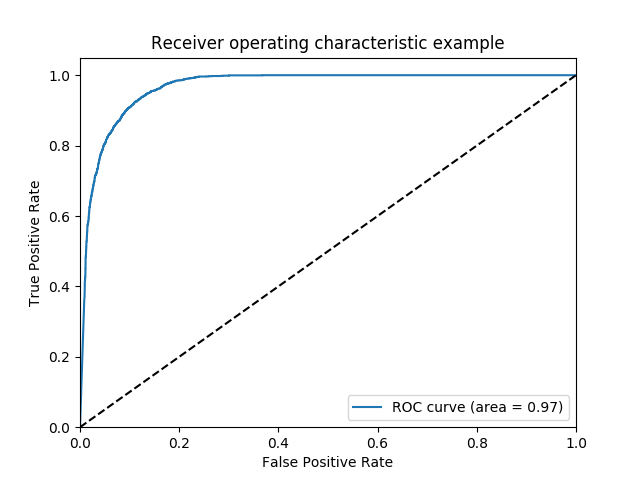
\includegraphics[width=10cm]{idiap_roc}
	\end{center}
	\caption[IDIAP database resulted ROC curve]{The resulted receiver operating characteristic curve for the IDIAP database corresponding to our implementation of a face spoof validator based on uniform LBP and linear SVM}
	\label{fig:idiap_roc}
\end{figure}
To produce the attacks, high-resolution photos and videos from each client were taken under the same conditions as in their authentication sessions, using a Canon PowerShot SX150 IS camera, which records both 12.1 Mpixel photographs and 720p high-definition video clips. The way to perform the attacks can be divided into two subsets: the first subset is composed of videos generated using a stand to hold the client biometry ("fixed"). For the second set, the attacker holds the device used for the attack with their own hands. In total, 20 attack videos were registered for each client, 10 for each of the attacking modes just described.
For the IDIAP database, we report an accuracy score of $0.91$, along with an EER of 0.09 and the confusion matrix being 
$
[
\begin{smallmatrix}
&Spoof & Real\\
Spoof & 5904 & 294\\
Real & 421 & 1679
\end{smallmatrix}] 
$. We present in figure \ref{fig:idiap_roc} the ROC curve.

\subsection{MSU USSA}
The Michigan State University Unconstrained Smartphone Spoof Attack Database consists of 9.000 images divided into 1.000 live subjects and 8.000 spoof attack. It was created having in mind that with the release of Android 4.0 millions of devices have the ability to be unlocked using the trusted face functionality therefore, in order to simulate the type of attacks that would challenge this method of security, the spoof attacks were captured using the front and rear camera of a Nexus 5. In order to create the database, 1.000 lives subject images of celebrities from the Weakly Labeled Face Database were selected and for each one four mediums of spoof attacks were recorder: MacBook, Nexus 5, Nvidia Shield Tablet and Printed Photo. 

The evaluation protocol of the MSU USSA database supposes to perform a five-fold subject exclusive cross-validation, each fold containing the one live subject image and its corresponding four spoof images. For each distinct fold, the other 4 folds are used to train the classifier. Performance is reported as the average EER and standard deviation across the five testing foldes. Therefore our classifier score a mean EER of $0.183$ with a standard deviation of $0.013$ with the following confusion matrices for eah of the five folds:
$
[
\begin{smallmatrix}
&Spoof & Real\\
Spoof & 1576 & 24\\
Real & 45 & 155
\end{smallmatrix}]
$, 
$
[
\begin{smallmatrix}
&Spoof & Real\\
Spoof & 1537 & 23\\
Real & 42 & 153
\end{smallmatrix}]
$
$
[
\begin{smallmatrix}
&Spoof & Real\\
Spoof & 1569 & 23\\
Real & 51 & 148
\end{smallmatrix}] 
$
$
[
\begin{smallmatrix}
&Spoof & Real\\
Spoof & 1526 & 26\\
Real & 38 & 156
\end{smallmatrix}] 
$
$
[
\begin{smallmatrix}
&Spoof & Real\\
Spoof & 1514 & 30\\
Real & 42 & 151
\end{smallmatrix}] 
$



\subsection{MSU MFSD}
Michigan State University Mobile Face Spoof Database was produced at the Michigan State University Pattern Recognition and Image Processing (PRIP) Lab, in East Lansing, US. and contains 280 video clips of photo and video attack attempts to 35 clients. As stated in the description of the database, it has the following properties:

\begin{itemize}
	\item Mobile phone is used to capture both genuine faces and spoof attacks, simulating the application of mobile phone unlock
	\item The printed photos used for attacks are generated with a state of the art color printer on larger sized paper. Hence, the printed photos in the MSU MFSD database have much better quality than the printed photos in the Idiap and CASIA databases.
\end{itemize}

Two types of cameras were used to collect the videos: built-in camera in MacBook Air 13” (640x480) and front-facing camera in the Google Nexus 5 Android phone (720x480). Three kinds of spoof medium were used to generate spoof attacks: high-resolution replay video attacks using an iPad Air screen, with resolution of 2048x1536, mobile phone replay video attacks using an iPhone 5S screen, with resolution of 1136x640, printed photo attacks using an A3 paper with fully-occupied printed photo of the client’s biometry, paper size: 11' x 17' (279mm x 432 mm), printed by a HP Color Laserjet CP6015xh printer, with printing resolution of 1200 x 600 dpi.
\begin{figure}[H]
	\captionsetup{width=15cm,font=small}
	\begin{center}
		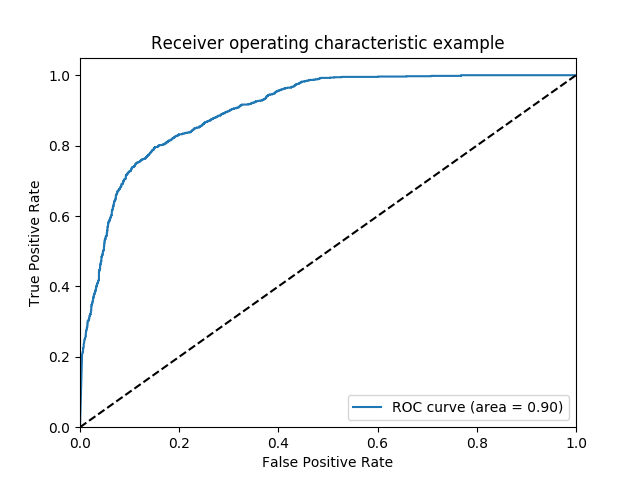
\includegraphics[width=10cm]{msu_mfsd}
	\end{center}
	\caption[MSU MFSD database resulted ROC curve]{The resulted receiver operating characteristic curve for the MSU MFSD database corresponding to our implementation of a face spoof validator based on uniform LBP and linear SVM}
	\label{fig:msu_mfsd}
\end{figure}

Our results on this database are as follows: the receiver operating characteristic can be seen in figure \ref{fig:msu_mfsd} with the AUC score of $0.903$ at an EER of $0.18$ with an accuracy score of $0.84$ and the confusion matrix 
$
[
\begin{smallmatrix}
&Spoof & Real\\
Spoof & 2677 & 410\\
Real & 244 & 799
\end{smallmatrix}] 
$



\subsection{Cross-database testing}\label{section:cross_database_testing}
Given that for each of the earlier presented databases, the train and test data were gathered using the same camera and spoof medium, we consider that a cross-database evaluation must also be done to get a better perspective on the reliableness of our implementation. Having at our disposal four databases with different collection parameters, we are able to run four tests where the data from three databases is used to train the SVM and then test it on the test data of the fourth. 
\begin{figure}[H]
	\captionsetup{width=15cm,font=small}
	\begin{center}
		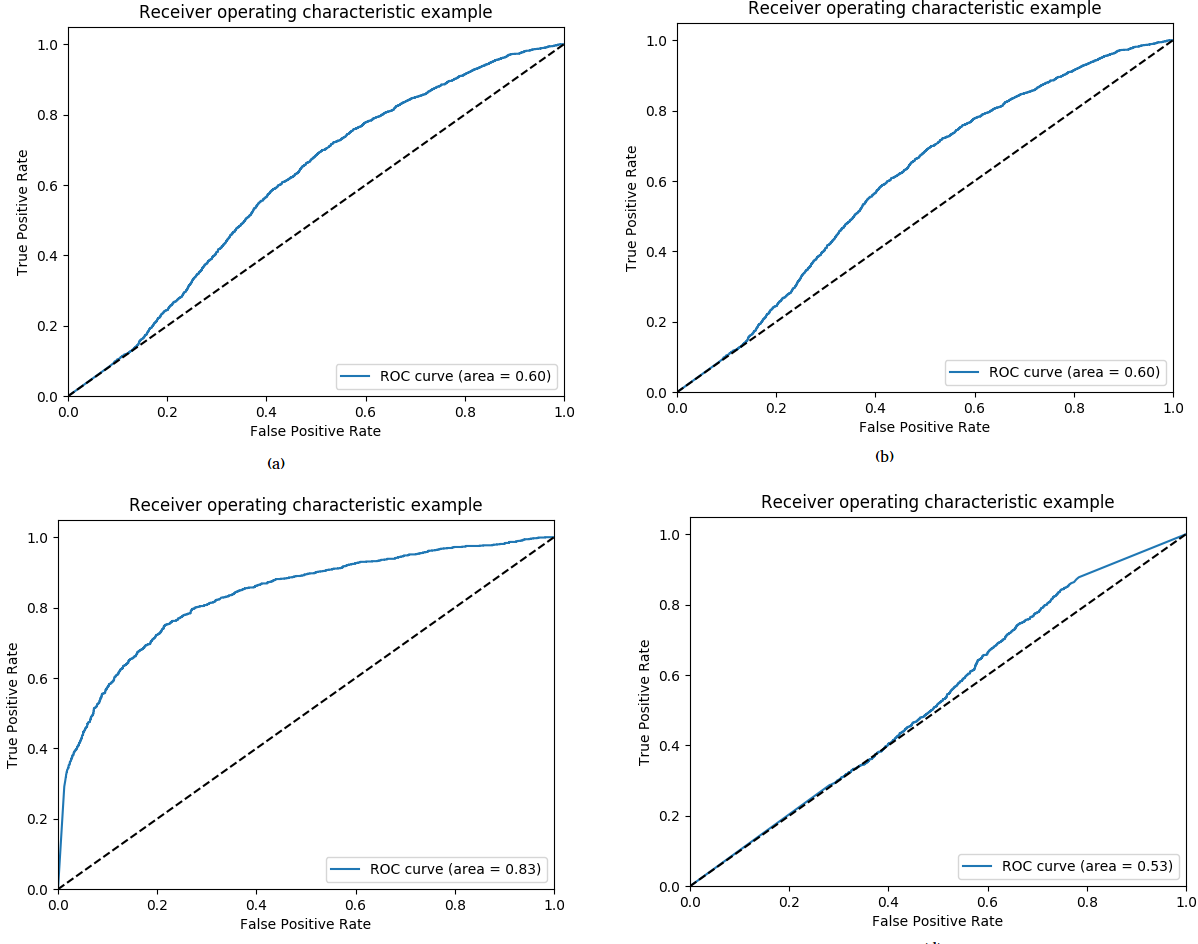
\includegraphics[width=15cm,height=10cm]{interdb_merged}
	\end{center}
	\caption[Cross-database face spoof classification results]{Here are presented the ROC curves for the four evaluations in the inter-database testing of CASIA, IDIAP, MSU USSA, MSU MFSD. (a) represents the ROC curve for the CASIA database when the IDIAP, MSU MFSD and MSU USSA databases are used as training data. (b) represents ROC curve for IDIAP when the other three are used as training data. (c) for MSU MFSD and (d) MSU USSA}
	\label{fig:interdb_results}
\end{figure}
In figure \ref{fig:interdb_results} can be observed the results of the four tests in the cross-database. As it can be seen, the results are quite disappointing compared to the intra-database evaluation of the efficiency of local binary patterns in detecting spoof faces. This makes us believe that the success of the LBP is highly dependent on the fact that the training and test data is collected with the same devices.

\section{Face distance threshold}
We now focus on determining the best value for the face distance threshold. As described in section \ref{face_recognition}, it represents the maximum distance between the embeddings of two faces at which we can still consider them as belonging to the same identity. We use a sample from the MS-Celeb-1M database of celebrities faces put together by Microsoft. It was gathered in order to create a benchmark task to recognize one million celebrities from their face images by using as training data all the face images of the individual that are available on the internet. Here we do three experiments in determining the threshold value based on the proposed approach in \ref{face_recognition}. The results can be seen in figure \ref{fig:face_distance_threshold}. 

\begin{figure}[H]
	\captionsetup{width=15cm,font=small}
	\begin{center}
		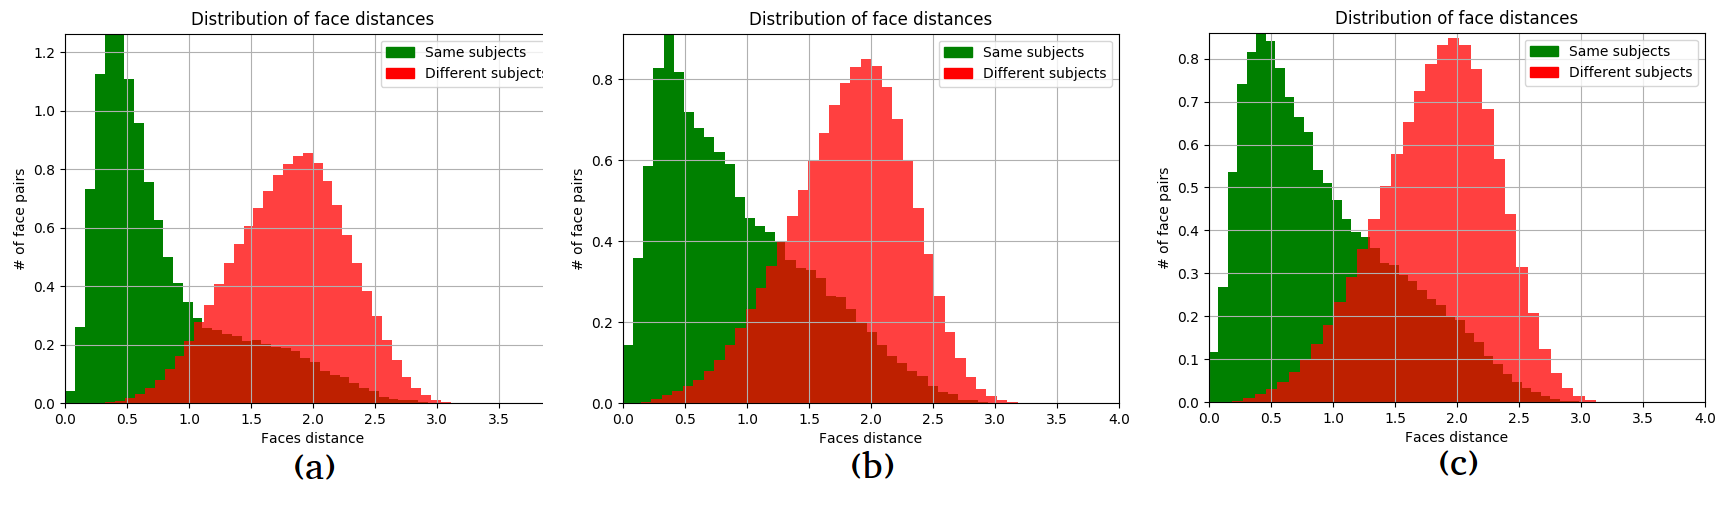
\includegraphics[width=15cm,height=7cm]{face_distance_threshold}
	\end{center}
	\caption[Faces distances histograms]{Here are the results for the three experiments: (a) corresponds to a selection of 14 identities with an average of 98 faces per identity. (b) is for 126 identities with an average of 20 faces per identity and (c) is the result for randomly sampling 315 identities with 28 faces per identity.}
	\label{fig:face_distance_threshold}
\end{figure}

\textbf{The first experiment} consists of randomly selecting \textbf{124} identities and for each one sampling in a random way about \textbf{28} faces. This produces a number of \textbf{2708} total face images from which we compute \textbf{3.660.000} pairs out of which \textbf{53.770} had the same identity and \textbf{3.606.230} had different identities. This produces a ratio of \textbf{0.15} same identity to different identities pairs.

We conduct \textbf{the second experiment} in the same way as the first one but with different number of subjects, specifically \textbf{316} and about \textbf{20} faces for every identity. This produces a number of \textbf{6320} total face images from which we compute \textbf{19.968.040} pairs out of which \textbf{60.040} had the same identity and \textbf{19.908.000} had different identities. This produces a ratio of \textbf{0.003} same identity to different identities pairs.

\textbf{The third experiment} differs from the first two in that we select a smaller number of identities but we increas the number of faces per identity. For this, we use the online available MS-Celeb-1M sample data containing \textbf{14} identities with approximately \textbf{98} faces per identity. Using this dataset, we had about \textbf{1.274} faces combined together in \textbf{810.901} pairs out of which \textbf{66.542} pairs with faces of the same identity and \textbf{744.359} with different identities, result in a ratio of \textbf{0.09} 	same identity to different identities pairs.


As a result of the three experiments, it can be seen in figure \ref{fig:face_distance_threshold} that the embedding function that produces the feature vector has a stable face distance threshold at around \textbf{1.1} which is invariant to number of identities and face images.
